\documentclass[12pt,fleqn]{article}\usepackage{../common}
\begin{document}
Dagilim Karisimlari ve Takip Edilmeden Kumeleme (Unsupervised Clustering)

Gaussian (normal) dagilimi tek tepesi olan (unimodal) bir dagilimdir. Bu
demektir ki eger birden fazla tepe noktasi olan bir veriyi modellemek
istiyorsak, degisik yaklasimlar kullanmamiz gerekecektir. 
Birden fazla Gaussian'i "karistirmak (mixing)" bu tur bir yaklasim
olabilir. Karistirmak, karisim icindeki her Gaussian'dan gelen sonuclari
toplamaktir, yani kelimenin tam anlamiyla her veri noktasini teker teker
karisimdaki tum dagilimlara gecip sonuclari toplamaktir. Eger cok boyutlu
normal dagilimlari topluyorsak, formul:

$$ p(x) = \sum_z \pi_z N(x | \mu_z,\Sigma_z) $$

$\pi_z$ karistirma oranlaridir (mixing proportions). Iki Gaussian oldugunu
dusunelim, $\pi_1,\pi_2$ oranlari 0.2, 0.8 olabilir mesela (toplam her
zaman 1 olmalidir), her nokta her Gaussian'a verildikten sonra tekabul eden
agirlikla mesela sirayla $0.2,0.8$ ile carpilip toplanir. 

Ornek olarak alttaki veriye bakalim.

\begin{minted}[fontsize=\footnotesize]{python}
def pnorm(x, m, s):
    """ 
    Compute the multivariate normal distribution with values
    vector x, mean vector m, sigma (variances/covariances) matrix
    s
    """
    xmt = np.matrix(x-m).transpose()
    for i in xrange(len(s)):
        if s[i,i] <= sys.float_info[3]: # min float
            s[i,i] = sys.float_info[3]
    sinv = np.linalg.inv(s)
    xm = np.matrix(x-m)
    return (2.0*math.pi)**(-len(x)/2.0)*\
        (1.0/math.sqrt(np.linalg.det(s)))\
        *math.exp(-0.5*(xm*sinv*xmt))

import scipy.stats
data = np.loadtxt('biometric_data_simple.txt',delimiter=',')

women = data[data[:,0] == 1]
men = data[data[:,0] == 2]

plt.xlim(55,80)
plt.ylim(80,280)
plt.plot (women[:,1],women[:,2], 'b.')
plt.hold(True)
plt.plot (men[:,1],men[:,2], 'r.')
plt.xlabel('height (inch)')
plt.ylabel('weight (pound)')
plt.savefig('mixbern_1.png')
\end{minted}

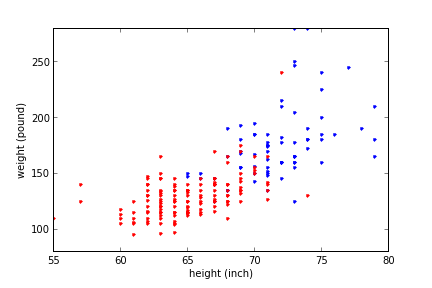
\includegraphics[height=6cm]{mixbern_1.png}

Bu grafik kadinlar ve erkeklerin boy (height) ve kilolarini (weight) iceren
bir veri setinden geliyor, veri setinde erkekler ve kadinlara ait olan
olcumler onceden isaretlenmis / etiketlenmis (labeled), biz de bu
isaretleri kullanarak kadinlari kirmizi erkekleri mavi ile grafikledik. Ama
bu isaretler / etiketler verilmis olsun ya da olmasin, kavramsal olarak
dusunursek eger bu veriye bir dagilim uydurmak (fit) istersek bir karisim
kullanilmasi gerekli, cunku iki tepe noktasiyle daha rahat temsil
edilecegini dusundugumuz bir durum var ortada.

\begin{minted}[fontsize=\footnotesize]{python}
# Multivariate gaussian, contours
#
import scipy.stats
data = np.loadtxt('biometric_data_simple.txt',delimiter=',')

def norm_pdf(b,mean,cov):
   k = b.shape[0]
   part1 = np.exp(-0.5*k*np.log(2*np.pi))
   part2 = np.power(np.linalg.det(cov),-0.5)
   dev = b-mean
   part3 = np.exp(-0.5*np.dot(np.dot(dev.transpose(),np.linalg.inv(cov)),dev))
   dmvnorm = part1*part2*part3
   return dmvnorm

women = data[data[:,0] == 1]
men = data[data[:,0] == 2]

plt.xlim(55,80)
plt.ylim(80,280)
plt.plot (women[:,1],women[:,2], 'b.')
plt.hold(True)
plt.plot (men[:,1],men[:,2], 'r.')
plt.xlabel('height (inch)')
plt.ylabel('weight (pound)')
plt.hold(True)

x = np.arange(55., 80., 1)
y = np.arange(80., 280., 1)
X, Y = np.meshgrid(x, y)

Z = np.zeros(X.shape)
nx, ny = X.shape
mu1 = np.array([  72.89350086,  193.21741426])
sigma1 = np.matrix([[    7.84711283,    25.03111826],
                    [   25.03111826,  1339.70289046]])
for i in xrange(nx):
    for j in xrange(ny):
        Z[i,j] = norm_pdf(np.array([X[i,j], Y[i,j]]),mu1,sigma1)
        
levels = np.linspace(Z.min(), Z.max(), 4)

plt.contour(X, Y, Z, colors='b', levels=levels)
plt.hold(True)

Z = np.zeros(X.shape)
nx, ny = X.shape
mu2 = np.array([  66.15903841,  135.308125  ])
sigma2 = np.matrix([[  14.28189396,   51.48931033],
                    [  51.48931033,  403.09566456]])
for i in xrange(nx):
    for j in xrange(ny):
        Z[i,j] = norm_pdf(np.array([X[i,j], Y[i,j]]),mu2,sigma2)
        
levels = np.linspace(Z.min(), Z.max(), 4)

plt.contour(X, Y, Z, colors='r', levels=levels)
plt.savefig('mixbern_2.png')
\end{minted}

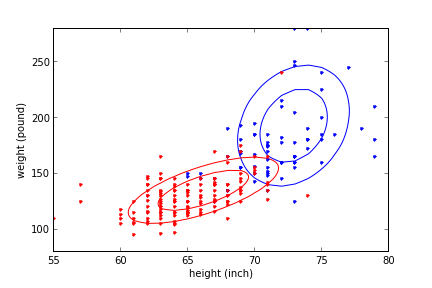
\includegraphics[height=6cm]{mixbern_2.png}

Bu karisim icindeki Gaussian'lari ustteki gibi cizebilirdik (gerci ustteki
aslinda ileride yapacagimiz net bir hesaptan bir geliyor, ona birazdan
geliyoruz, ama ciplak gozle de bu sekil uydurulabilirdi). Modeli kontrol
edelim, elimizde bir karisim var, nihai olasilik degeri $p(x)$'i nasil
kullaniriz? Belli bir noktanin olasiligini hesaplamak icin bu noktayi her
iki Gaussian'a teker teker geceriz (ornekte iki tane), ve gelen olasilik
sonuclarini karisim oranlari ile carparak toplariz.
Agirliklar sayesinde iki sey elde ediyoruz 1) karisim entegre edilince hala
1 degeri cikiyor zaten bir dagilimin uymasi gereken sartlardan biri bu 2)
kesisim olan bolgelerde her iki Gaussian buyuk bir deger verebilir, o zaman
agirliklar devreye girer, ve nihai olasilik, agirliklara gore carpilip
toplanan bir sonuc olur. Bu bolgelerde bir Gaussian'in agirliginin
digerinden fazla olmasinin da ozel bir anlami var, demek ki o bolgede
agirligi fazla olan Gaussian daha fazla noktaya sahip (verisel olarak), ki
o zaman o bolgedeki bir noktanin olasiligi sorulunca, agirligi fazla olan
Gaussian daha yuksek bir olasilik degeri geri dondurmeli.

Kesisme olmayan bolgeler zaten pek onemli degil, o noktalarin olasilik
degeri zaten agirlikla tek bir Gaussian'dan geliyor olacak, cunku diger
Gaussian o bolge icin sifira yakin bir deger verir, ve bu sifira yakin
deger toplamda zaten bir fark yaratmayacak.

Etiketler Bilinmiyorsa

Simdi veriyi modellemenin otesinde, biraz daha analitik, daha makine
ogrenimi ile alakali ihtiyaclara gelelim. Eger etiketler bize onceden
verilmemis olsaydi, hangi veri noktalarinin kadinlara, hangilerinin
erkeklere ait oldugunu bilmeseydik o zaman ne yapardik? Bu veriyi
grafiklerken etiketleri renkleyemezdik tabii ki, soyle bir resim
cizebilirdik ancak,

\begin{minted}[fontsize=\footnotesize]{python}
import scipy.stats
data = np.loadtxt('biometric_data_simple.txt',delimiter=',')

women = data[data[:,0] == 1]
men = data[data[:,0] == 2]

plt.xlim(55,80)
plt.ylim(80,280)
plt.plot (data[:,1],data[:,2], 'k.')
plt.xlabel('height (inch)')
plt.ylabel('weight (pound)')
plt.savefig('mixbern_3.png')
\end{minted}

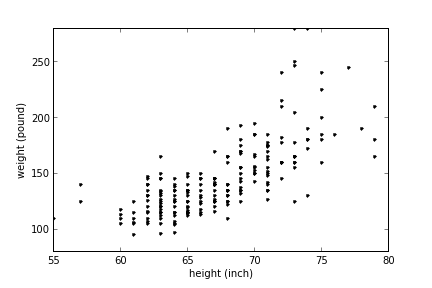
\includegraphics[height=6cm]{mixbern_3.png}

Fakat yine de sekil olarak iki kumeyi gorebiliyoruz. 
Acaba oyle bir makine ogrenimi algoritmasi olsa da, biz bir karisim
oldugunu tahmin edip, sonra o karisimi veriye uydururken, etiket
degerlerini de kendiliginden tahmin etse? Bu tam bir veri madenciligi
denemesi olurdu.

Bu ise baslamadan once etiketler ile karisimlarin arasindaki baglantiyi
gorelim. Her nokta icin bilinen / bilinmeyen etiket kavramindan,
matematiksel olarak direk karisimlara gecis yapabilmemiz lazim.

Diyelim ki her nokta icin $0/1$ degerini tasiyabilecek "gizli" bir $z$
rasgele degiskeni var, o zaman $p(x)$'i su sekilde acabiliriz

$$ p(x) = \sum_z p(x,z) $$

Bu mantikli degil mi? Ortak dagilim $p(x,z)$ icinden $p(x)$'i cekip
cikarmak, $p(x,z)$ icin bir bilesen (marginal) hesabi yapmak demektir, o
zaman ortak dagilimin icindeki tum $z$ degerlerini toplamak gerekir. Devam
edelim, Bayes Teorisi'ni kullanarak

$$ = \sum_z p(x,z) = \sum_z  p(z)p(x|z) $$

elde ederiz. Burada $p(z)$, yani $z$'nin 0/1 degerine "sahip olup
olmadiginin olasiligi" bizi $\pi_z$'ye goturur, yani

$$ \sum_z  p(z)p(x|z) = \sum_z  \pi_zN_z(x | \mu_z,\sigma_z) $$

Unutmayalim, $z$ bir rasgele degisken, ve sahip oldugu olasiliga gore, her
veri noktasi icin, 0 ya da 1 uretiyor. $p(z)$ dedigimiz zaman $z$ tek
basina, baska hicbir parametre ona gecilmiyor, o zaman zaten tanim
itibariyle "ta en bastan belirli" bir olasiliktan baska bir seye sahip
olamaz, bu da karisim orani $\pi_z$'den baskasi degildir. 

Notasyon

Simdi notasyonu biraz daha berraklastiralim. Oncelikle, ozellikle Bayes
modelleri iceren formulasyonlarda, $p(x)$, $p(z)$ gibi kullanimlar gorulur,
fakat aslinda orada iki tane farkli yogunluk fonksiyonu (density function)
kastedilir, $p_x(x)$ ve $p_z(z)$. Surekli $p$ kullanilan turden kullanimin
biraz ustunkoru (sloppy) oldugu dogrudur, kimisi icin bu daha kisa yoldan
formulasyondur, literaturu takip eden herkes bunun nereden geldigini bilir,
sadece konuya ilk baslayanlar icin biraz kafa karistirici olabiliyor.

Ayrica $p(z)$ derken $p(z=k)$ demek istiyoruz, yani 

$$ p(x) = \sum _{ k=1}^{K} p(z=k)p(x | z=k) $$

ki $K$ karisimdaki Gaussian sayisidir. Aynen ustte oldugu gibi etiketin
bilindigi, "verili" oldugu durumda kosullu olasilik $p(x | z=k)$,
karisimdaki Gaussian'lardan bir tanesidir, ki o da ustte $N_z(x |
\mu_z,\sigma_z)$ 
olarak gosterilmisti, simdi $k$ kullanirsak $N(x |
\mu_k,\sigma_k)$ olacaktir.

Iki Gaussian oldugu durumda $z$'nin 0/1 degerine sahip olup olmadigindan
bahsettik, ya da $K$ ikiden daha buyuk oldugu durumlarda, $z = k$ olup
olmama durumu. Aslinda bir temsili yontem daha var, $z$ rasgele degiskenini
sadece bir hucresinde 1 ya da 0 tasiyan bir katl� terimli (multinomial)
dagilim, yani bir vektor olarak gostermek. Yani $z = [0 \ 0 \ 1 \ .. \ 0 ]^T$
seklinde. Bu temsili yonteme K-icinde-1 (1-of-K) temsili yontemi deniyor. O
zaman 

$$ p(z) = \prod _{ k=1}^{K}\pi_k ^{z_k} 
\mlabel{1}
$$

ve

$$ p(x | z) = \prod _{ k=1}^{K} N(x | \mu_k,\Sigma_k)^{z_k} 
\mlabel{2}
$$

Peki verinin log olabilirligi (log likelihood) nedir? 

Bilindigi gibi olabilirlik hesap veri noktalarinin teker teker yogunluk
fonksiyonuna gecilmesi, ve sonuclarin birbiri ile carpilmasidir, log
olabilirlik ise onun log alinmis halidir (cunku log alininca carpimlar
toplam haline donusur, boylece mutlak (absolute) olarak gittikce buyuyen
bir sayi ile islem yapilabilir, oteki turlu olasilik degeri oldugu icin
1'den kucuk sayilarin surekli birbiri ile carpimi, nihai carpimi asiri
kucultur, bu da bilgisayarin numerik hesap sinirlarini zorlayabilir. 

$X$'i tum $x$'leri iceren bir matrix olarak kabul edelim

$$ \ln p(X|\pi,\mu,\Sigma) = \sum _{n=1}^{N} 
\ln 
\bigg\{
\sum _{ k=1}^{K}
\pi_k p(x_n | \mu_k,\Sigma_k)\
\bigg\}
$$

Genellikle olabilirlik fonksiyonu maksimize edilerek icindeki
parametrelerin bu maksimum noktada tasidigi degerler bulunmaya
ugrasilir. Fakat bizim esas ilgilendigimiz "bilinmeyen" etiketler, o
yuzden maksimizasyon yapmadan once bu etiketleri de bir sekilde
olabilirligin icine dahil etmemiz lazim. (1) ve (2)'yi kullanirsak, 

$$ p(X,Z | \mu,\Sigma,\pi) =
\prod _{n=1}^{N}
\prod _{k=1}^{K}
\pi_k ^{z_{nk}} N(x_n|\mu_k,\Sigma_k)
 $$

Bunun log'unu alirsak

$$ \ln p(X,Z | \mu,\Sigma,\pi) =
\ln
\sum _{n=1}^{N}
\sum _{k=1}^{K}
z_{nk} \{ \ln \pi_k + \ln N(x_n|\mu_k,\Sigma_k) \}
 $$

EM (Expectation Maximization) metotu, bu olurluk fonksiyonunu baz alarak,
$\mu,\Sigma,\pi$ bilindigi durumda etiketleri, etiketler bilindigi durumda
$\mu,\Sigma,\pi$ degerlerini tahmin eder, bu iki bilinmeyen grup arasinda
ozyineli (iteratif) olarak gidip gelir. Tabii konunun cok fazla detayi var [1],
oncelikle EM'in ustteki durumda yakinsak (convergence) bir davranis
sergiledigi bilinir, yani bir optimum vardir, va belli uc nokta sartlari
haricinde bu degere yaklasilmasi garantidir, vs.

\begin{minted}[fontsize=\footnotesize]{python}
import math, random, copy, sys

def expectation_maximization(t, nbclusters=2, nbiter=3, \
                                 normalize=False,epsilon=0.001, \
                                 monotony=False, datasetinit=True):
    def draw_params():
            if datasetinit:
                tmpmu = np.array([1.0*t[random.uniform(0,nbobs),:]],
                                 np.float64)
            else:
                tmpmu = np.array([random.uniform(min_max[f][0],
                                                 min_max[f][1])\
                        for f in xrange(nbfeatures)], np.float64)
            return {'mu': tmpmu,\
                    'sigma': np.matrix(np.diag(\
                    [(min_max[f][1]-min_max[f][0])/2.0\
                    for f in xrange(nbfeatures)])),\
                    'proba': 1.0/nbclusters}

    nbobs = t.shape[0]
    nbfeatures = t.shape[1]
    min_max = []
    # find xranges for each features
    for f in xrange(nbfeatures):
        min_max.append((t[:,f].min(), t[:,f].max()))
    
    ### Normalization
    if normalize:
        for f in xrange(nbfeatures):
            t[:,f] -= min_max[f][0]
            t[:,f] /= (min_max[f][1]-min_max[f][0])
    min_max = []
    for f in xrange(nbfeatures):
        min_max.append((t[:,f].min(), t[:,f].max()))
    ### /Normalization

    result = {}
    quality = 0.0 # sum of the means of the distances to centroids
    random.seed()
    Pclust = np.ndarray([nbobs,nbclusters], np.float64) # P(clust|obs)
    Px = np.ndarray([nbobs,nbclusters], np.float64) # P(obs|clust)
    # iterate nbiter times searching for the best "quality" clustering
    for iteration in xrange(nbiter):
        # Step 1: draw nbclusters sets of parameters #
        params = [draw_params() for c in xrange(nbclusters)]
        old_log_estimate = sys.maxint         # init, not true/real
        log_estimate = sys.maxint/2 + epsilon # init, not true/real
        estimation_round = 0
        # Iterate until convergence (EM is monotone) <=>
        # < epsilon variation
        while (abs(log_estimate - old_log_estimate) > epsilon\
                and (not monotony or log_estimate < old_log_estimate)):
            restart = False
            old_log_estimate = log_estimate
            # Step 2: compute P(Cluster|obs) for each observations #
            for o in xrange(nbobs):
                for c in xrange(nbclusters):
                    # Px[o,c] = P(x|c)
                    Px[o,c] = pnorm(t[o,:],\
                            params[c]['mu'], params[c]['sigma'])
            #for o in xrange(nbobs):
            #    Px[o,:] /= math.fsum(Px[o,:])
            for o in xrange(nbobs):
                for c in xrange(nbclusters):
                    # Pclust[o,c] = P(c|x)
                    Pclust[o,c] = Px[o,c]*params[c]['proba']
            #    assert math.fsum(Px[o,:]) >= 0.99 and\
            #            math.fsum(Px[o,:]) <= 1.01
            for o in xrange(nbobs):
                tmpSum = 0.0
                for c in xrange(nbclusters):
                    tmpSum += params[c]['proba']*Px[o,c]
                Pclust[o,:] /= tmpSum
                #assert math.fsum(Pclust[:,c]) >= 0.99 and\
                #        math.fsum(Pclust[:,c]) <= 1.01
            # Step 3: update the parameters (sets {mu, sigma, proba}) #
            #print "iter:", iteration, " estimation#:", estimation_round,\
            #        " params:", params
            for c in xrange(nbclusters):
                tmpSum = math.fsum(Pclust[:,c])
                params[c]['proba'] = tmpSum/nbobs
                # restart if all converges to one cluster
                if params[c]['proba'] <= 1.0/nbobs:  
                    restart = True                   
                    #print "Restarting, p:",params[c]['proba'] 
                    break
                m = np.zeros(nbfeatures, np.float64)
                for o in xrange(nbobs):
                    m += t[o,:]*Pclust[o,c]
                params[c]['mu'] = m/tmpSum
                s = np.matrix(np.diag(np.zeros(nbfeatures, np.float64)))
                for o in xrange(nbobs):
                    s += Pclust[o,c]*\
                    (np.matrix(t[o,:]-params[c]['mu']).transpose()*\
                     np.matrix(t[o,:]-params[c]['mu']))
                params[c]['sigma'] = s/tmpSum
                #print "------------------"
                #print params[c]['sigma']

            ### Test bound conditions and restart consequently if needed
            if not restart:
                restart = True
                for c in xrange(1,nbclusters):
                    if not np.allclose(params[c]['mu'],
                                       params[c-1]['mu'])\
                    or not np.allclose(params[c]['sigma'],
                                       params[c-1]['sigma']):
                        restart = False
                        break
            if restart:     # restart if all converges to only
                old_log_estimate = sys.maxint     # init, not true/real
                log_estimate = sys.maxint/2 + epsilon # init, not true/real
                params = [draw_params() for c in xrange(nbclusters)]
                continue
            ### /Test bound conditions and restart

            # Step 4: compute the log estimate #
            log_estimate = math.fsum([math.log(math.fsum(\
                    [Px[o,c]*params[c]['proba'] \
                         for c in xrange(nbclusters)]))\
                                          for o in xrange(nbobs)])
            #print "(EM) old and new log estimate: ",\
            #        old_log_estimate, log_estimate
            estimation_round += 1

        # Pick/save the best clustering as the final result
        quality = -log_estimate
        if not quality in result or quality > result['quality']:
            result['quality'] = quality
            result['params'] = copy.deepcopy(params)
            result['clusters'] = [[o for o in xrange(nbobs)\
                    if Px[o,c] == max(Px[o,:])]\
                    for c in xrange(nbclusters)]
    return result

data = np.loadtxt('biometric_data_simple.txt',delimiter=',')
data = data[:,1:3]
res = expectation_maximization(data)
print res
\end{minted}

\begin{verbatim}
{'params': [{'mu': array([  66.12666308,  135.12466099]), 'sigma': matrix([[  14.13415772,   50.64636849],
        [  50.64636849,  397.62384374]]), 'proba': 0.8166232863917395}, {'mu': array([  72.86275108,  192.56097154]), 'sigma': matrix([[    7.88624494,    25.75436975],
        [   25.75436975,  1336.81524343]]), 'proba': 0.1833767136082604}], 'quality': 1523.0485855071697, 'clusters': [[0, 1, 2, 3, 4, 5, 7, 8, 9, 10, 13, 14, 15, 16, 17, 18, 19, 20, 21, 22, 25, 26, 27, 28, 29, 30, 31, 32, 33, 35, 36, 37, 39, 40, 42, 43, 46, 48, 49, 51, 52, 54, 57, 58, 59, 61, 63, 64, 65, 66, 68, 69, 70, 72, 73, 74, 75, 79, 80, 81, 82, 83, 84, 86, 87, 88, 89, 90, 91, 92, 93, 94, 95, 96, 97, 103, 105, 107, 108, 109, 110, 111, 112, 113, 114, 115, 119, 120, 121, 122, 123, 124, 128, 132, 133, 134, 135, 137, 138, 139, 140, 142, 143, 145, 146, 147, 148, 149, 151, 152, 153, 154, 156, 157, 158, 159, 161, 162, 163, 164, 165, 166, 168, 170, 171, 172, 174, 175, 176, 177, 178, 179, 180, 182, 183, 185, 186, 187, 189, 190, 192, 193, 194, 195, 196, 197, 198, 200, 201, 202, 203, 208], [6, 11, 12, 23, 24, 34, 38, 41, 44, 45, 47, 50, 53, 55, 56, 60, 62, 67, 71, 76, 77, 78, 85, 98, 99, 100, 101, 102, 104, 106, 116, 117, 118, 125, 126, 127, 129, 130, 131, 136, 141, 144, 150, 155, 160, 167, 169, 173, 181, 184, 188, 191, 199, 204, 205, 206, 207, 209]]}
\end{verbatim}

Ustteki kod \verb!biometric_data_simple.txt! verisi uzerinde isletildiginde
rapor edilen $\mu,\Sigma$ degerlerini grafikleyince basta paylastigimiz
grafik goruntuleri cikacaktir, yani kumeleme basariyla isletilmistir.  Cok
Degiskenli Bernoulli Karisimi (Mixture of Multivariate Bernoulli)

Bir karisim Gaussian'lardan olustugu gibi, degisik dagilimlardan da
mutesekkil olabilir. Mesela her biri 8x8 boyutlarda ve 64 ogeli duz bir
vektor olarak temsil edilen, icinde ikisel (binary) veri tasiyan, yani
siyah / beyaz olarak temsil edilen karakterleri gruplama problemini ele
alalim.

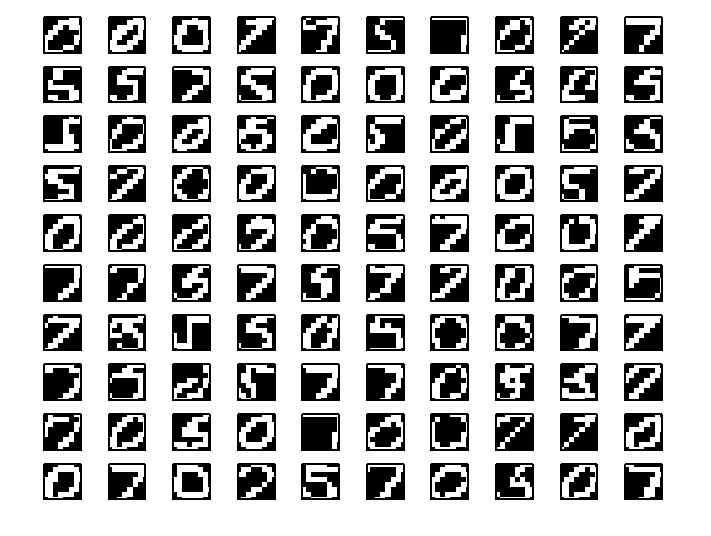
\includegraphics[height=6cm]{digits.png}

Bu karakterlerin hepsini \verb!bindigit.py! ile sirayla
gorebilirsiniz. Mesela ust soldan saga dogru giderken 3 tane sifira benzer
karakter goruyoruz, sonra yediye benzer iki goruntu goruyoruz, vs. Burada
temsil etmemiz gereken, demek ki, bu 64 hucreli sadece 1 ve 0 degeri
tasiyan degerleri temsil etmek. Boy ve agirlikta iki hucreli vektorde
sadece reel sayilar vardi. Simdi 64 hucreli vektorde ikisel degerler var. 
Boyle bir veriyi hangi dagilim en iyi temsil eder? Sadece tek 1 ve 0
olsaydi, o zaman Bernoulli dagilimi kullanirdik,

$$ p(x) = \alpha^x(1-\alpha)^{1-x} $$

$\alpha$ bu dagilimi tanimlayan 0 ve 1 arasinda bir degerdir. 

Bernoulli'leri cok degiskenli olarak kullanamaz miyiz? Kullaniriz.

$$ p(x) = \prod _{ d=1}^{D} \alpha_d^{x_d}(1-\alpha_d)^{1-x_d} $$

Bu durumda $x$ cok boyutlu, $D$ boyutlu bir vektor, yani $[0 \ 1 \ 1 \ 0 \
... \ 1]$ 
seklinde olacak. 

Eger cok degiskenli Bernoulli'lerin karisimini elde etmek istiyorsak,
$p(x|z)$ Gaussian yerine cok degiskenli Bernoulli olacak, yani

$$ p(x|z) = \prod _{ d=1}^{D} \alpha_{zd}^{x_d}(1-\alpha_{zd})^{1-x_d} $$

$\alpha_{zd}$, karisimdaki $z$'inci dagilimin $d$'inci hucresindeki olasilik degerini 
verecektir. Tum karisimin dagilimi daha once oldugu gibi

$$ p(x) = \sum_z  p(z)p(x|z)$$ 

Suna dikkat etmek lazim -- karisim deyince mesela $[0 \ 1 \ 1 \ ... \ 1]$
vektoru ile $[1 \ 0 \ 1 \ ... \ 1]$ vektorunu "toplayip" yeni bir vektor elde
etmiyoruz. Bu vektorleri tum karisimin yogunlugu $p(x)$'e gecince bize bir
olasilik degeri veriliyor. Bunun hesaplanisi, perde arkasinda teker teker
karisimdaki tum bilesenlerin yogunluguna teker teker sormak, ve geriye bir
cevap vermeden once agirligi kullanarak dengelemek. 

Ya da uretimsel (generative) olarak olaya bakarsak, $p(x)$'in temsil ettigi
yogunluga "zar attirarak" ile $[1 \ 1 \ 1 \ ... \ 0]$, $[1 \ 0 \ 0 \
... \ 0]$ gibi vektorler 
urettiriyor olabilirdik. Tabii ki bu uretim yogunlugun kontrolunde olarak, 
daha olasi turden vektorlerin, daha fazla ortaya cikmasi anlamina
gelecekti. 

Uretimsel derken, her veri noktasi icin bu uretimsel algoritmanin tamami
soyle:


for  i = 1  to N

$\ \ \ $ Olasilik vektoru $\pi$'ye gore zar at

$\ \ \ $ Sonuca  gore $m \leftarrow M$  modelden bir tanesini sec

$\ \ \ $ O modele $N(x_i|\mu_m,\Sigma_m)$ (ya da onun Bernoulli karsiligi) $x_i$


Altta yine EM kullanarak gruplama yapan yani etiketleri otomatik olarak
bulan kodu sunuyoruz. En sonda \verb!np.argmax(lR.T,axis=0)! ifadesini
goreceksiniz. \verb!lR!, \verb!NxD! boyutlu bir matristir, her veri
noktasinin $D$ kumenin her birine olan aidiyatini olasilik degeri olarak
tasir, \verb!argmax! ifadesi satirsal bazda bu aidiyatlarin en buyugunun
"indisini" dondurur, eger 3 tane kume var demissek, o zaman 

\verb![1 1 1 0 2 0 2 ... ]!

gibi bir sonuc gorulecektir. Demek ki 1. nokta 1. kumeye, 4. nokta
0. kumeye aittir. Hakikaten de basta paylastigimiz resimlere
bakarsaniz, ilk 3 karakterin birbirine benzedigi farkedilecektir.

Sonuc olarak verdigimiz bu algoritmalar idare edilmeyen (unsupervised)
algoritmalar olarak bilinir, cunku algoritma "kendi basina" giderek
noktalarin hangi kumeye ait oldugunu hesaplamaktadir. Idare edilen
(supervised) yontemlerde oldugu gibi bir onceden isaretlenmis ornekler
yoktur.

Ne Zaman EM, Ne Zaman MCMC?

Bayes Teorisi ile sofistike olasiliksal modeller olusturulabilir ve bu
modellerin hepsi MCMC ile hesaplanabilir, cozulebilir. Peki ne zaman EM
kullanilmali, ne zaman MCMC kullanmali.

Bu noktada Makine Ogrenimi alaninda unlu bir hoca Kevin Murphy'nin sozunu
hatirlamak iyi olabilir, demistir ki "EM fakir adamin Bayes
metotudur". EM her yerde kullanilamayabilir, ama kullanilabiliyorsa cabuk
isledigi bilinir, ve probleme uygulanmasi basittir. Probleminizde
karisimlar var ise, etiketleme yapiliyorsa, EM ilk akla gelen yontemlerden
biri olabilir. Tabii ki karisimlar ve diger her tur Bayes problemi MCMC ile
de hesaplanabilir.

\begin{minted}[fontsize=\footnotesize]{python}
def loginnerprodexp(t,a):
    eps=1e-15
    t[t>0.] = 1
    tmp = np.dot(t,np.exp(a)) + eps
    b=np.log(tmp)
    return b

def logsumexp(a):
    return np.log(np.sum(np.exp(a), axis=0))

def EMmixtureBernoulli(Y,K,iter,tol):
    N,D=Y.shape
    OMY=1+(-1*Y) #  "One minus Y", (1-Y)
    tmp=np.random.rand(N,K)
    tmp2=np.sum(tmp,axis=1).reshape((N,1))
    tmp3=np.tile(tmp2,(1,K))
    lR=np.log(np.divide(tmp, tmp3))
    L = []
    for i in range(iter):
        # lPi log Mixture params Kx1
	lPi=np.tile(-1 * np.log(N),(K,1))+logsumexp(lR).T.reshape((K,1))
        const=np.tile(logsumexp(lR).T.reshape((K,1)),(1,D))
        # lP log Bernoulli params KxD
        lP=loginnerprodexp(Y.T,lR).T - const
        # lOMP log(1-P), also KxD
        lOMP=loginnerprodexp(OMY.T,lR).T-const
	
	# *** E-step        
	lR=np.tile(lPi.T,(N,1))+np.dot(Y,lP.T) + np.dot(OMY,lOMP.T) # + const
        Z=logsumexp(lR.T)

        lR=lR-np.tile(Z.T.reshape((N,1)),(1,K))
        L.append(np.sum(Z))
        if (i>1):
            if np.abs(L[i]-L[i-1]) < tol: break

    iters = i
    return lR,lPi,lP,L,iters

import matplotlib.image as mpimg

K=3
iter=20
Y = np.loadtxt('binarydigits.txt')

attempts=20
Lbest = -np.inf
eps=1e-15
for attempt in range(attempts):
    lRtmp,lPitmp,lPtmp,L,iters = EMmixtureBernoulli(Y,K,iter,eps)
    if L[iters]>Lbest:
        lR=lRtmp
        lPi=lPitmp
        lP=lPtmp
        Lbest=L[iters]
        itersbest=iters

# show class labels
labels =  np.argmax(lR.T,axis=0)
print labels
\end{minted}

\begin{verbatim}
[0 0 0 2 1 2 1 0 2 1 2 2 1 2 0 0 0 2 0 2 2 0 0 2 0 2 0 2 2 2 2 2 0 0 0 0 0
 0 2 2 0 0 0 0 0 2 1 0 0 2 1 1 2 1 2 2 2 0 0 2 2 2 2 2 0 2 0 0 1 2 1 2 0 2
 1 1 0 2 2 2 1 0 2 0 1 0 0 2 2 0 0 1 0 1 2 1 0 2 0 1]
\end{verbatim}

Elde edilen sonuclara gore, ve paylastigimiz say resimlerindeki siraya
bakarsak, mesela ilk uc sayi imajini birbirine benziyor olmasi lazim.
Yine ayni sirada gidersek Daha sonra 4. ve 6. sayilarin birbirine
benziyor olmasi lazim, ve 8. imajin ilk uc imaja benziyor olmasi
lazim, vs. Resimlere bakinca bunun hakikaten boyle oldugunu
goruyoruz. Demek ki kumeleme basariyla gerceklestirilmis.

[1] Aaron A. D'Souza, Using EM To Estimate A Probablity Density With A
Mixture Of Gaussians, \url{http://www-clmc.usc.edu/~adsouza/notes/mix_gauss.pdf}

[2] Bernoulli mixture models for binary images, Alfons Juan, Enrique Vidal

[3] Jebara, T., Machine Learning Lecture Notes

[4] Iain Murray's Octave code on mixture of multivariate bernoullis

[5] \url{http://code.activestate.com/recipes/577735-expectation-maximization/download/1/}

[6] Bishop, C., Pattern Recognition and Machine Learning

[7] \url{http://ascratchpad.blogspot.de/2010/01/porting-code-from-matlab-octave-to.html}

[8] \url{http://www.scipy.org/NumPy_for_Matlab_Users/}

[9] \url{http://mathesaurus.sourceforge.net/matlab-numpy.html}


\end{document}
